\documentclass[a4paper, 11pt]{article}
\usepackage[letterpaper,margin=0.8in]{geometry}
\usepackage{blindtext}
\usepackage{lastpage}
\usepackage{fancyhdr}
\usepackage{xcolor}
\usepackage{setspace}
\usepackage{amsmath}
\usepackage{graphicx}
\usepackage{matlab-prettifier}
\usepackage{float}
\usepackage[small,bf,hypcap=true]{caption}

\newenvironment{Figure}
  {\par\medskip\noindent\minipage{\linewidth}
   \captionsetup{type=figure}}
  {\endminipage\par\medskip}
\usepackage[hidelinks]{hyperref}
\usepackage{titlesec}
\usepackage{tocloft}

\renewcommand{\cftsecleader}{\cftdotfill{\cftdotsep}}

\graphicspath{{./Figures}}

% Configure the header
\pagestyle{fancy} % Enable fancy headers
\fancyhead[L]{CE 593} % Left-aligned header
\fancyhead[C]{Statistical Analysis in Coastal Engineering} % Centered header
\fancyhead[R]{24/10/2025} % Right-aligned header

\setlength{\floatsep}{6pt plus 2pt minus 2pt}      % space between floats
\setlength{\textfloatsep}{8pt plus 2pt minus 2pt}  % space between floats and text
\setlength{\intextsep}{8pt plus 2pt minus 2pt}     % space above and below in-text floats

\onehalfspacing

\begin{document}

\titleformat{\section}
  {\normalfont\bfseries\fontsize{12}{10}\selectfont}
  {\large\thesection.} 
  {0.3em}
  {}

\thispagestyle{empty}

\begin{figure}[H]
    \vspace{0.6cm}
    \centering
    
\includegraphics[width=0.45\textwidth]{logo.png}
\end{figure}
\vspace{0.8cm}

\begin{center}
    \textbf{\LARGE Middle East Technical University}
    \vspace{0.3cm}

    \textbf{\LARGE Department of Civil Engineering}
    \vspace{0.5cm}

    \textbf{\Large 2025-2026 Fall Semester}
    \vspace{1.5cm}

    \textbf{\Large CE593 Statistical Analysis in Coastal Engineering}
    \vspace{0.9cm}

    \textbf{\LARGE Homework \#2}
    \vspace{1.5cm}

    \large Instructor:

    \large Assoc.Prof.Dr. Cüneyt Baykal
    \vspace{1.2cm}

    \large Submitted by:
    
    \large Bilge Kutay

    \large 2511798

\end{center}

\newpage
\renewcommand{\contentsname}{Table of Contents} 
\begin{center}
    \tableofcontents
\end{center}
\newpage

\listoffigures
\newpage

\section{Introduction}

\hspace*{0.5cm}Random sea waves observed in the ocean can be represented as a superposition of linear wave components with different frequencies, amplitudes, and directions. Each wave component contributes to the overall sea surface elevation, and the combined effect results in a random complex surface profile. 

In this assignment, a MATLAB routine was developed to generate and visualize the surface elevation of random sea waves based on a specified wave spectrum. The Pierson-Moskowitz (PM) spectrum, which describes the energy distribution of fully developed sea states, was used as the basis for generating the wave components. 

The aim of this study is to demonstrate how a random wave field can be created from a known spectrum and to visualize the resulting sea surface elevation over a specified spatial domain. 

\section{Methodology}

\hspace*{0.5cm}The sea surface was modeled as the sum of $N$ sinusoidal wave components where $N = 50$ is the number of frequency components, $f_i$ are the wave frequencies between $0.1\,\mathrm{Hz}$ and $10\,\mathrm{Hz}$, $a_i$ are the amplitudes, and $\varepsilon_i$ are random phases uniformly distributed between $0$ and $2\pi$ (\autoref{eq:surface_elevation}).

\begin{equation}
    \eta(t) = \sum_{i=1}^{N} a_i \cos(2 \pi f_i t + \varepsilon_i)
    \label{eq:surface_elevation}
\end{equation}

The amplitude of each component was obtained from the Pierson-Moskowitz spectrum (\autoref{eq:pm_spectrum}), which is defined as:
\begin{equation}
    a_i = 2\Delta f [0.205A^2B^{-4}f_i^{-5} \exp(-0.75(Bf_i)^{-4})]\phi(\omega_i)
    \label{eq:pm_spectrum}
\end{equation}

where $A = 0.15, B = 1.6, \omega_i = 2\pi f_i$ and $\phi(\omega_i)$ is a correction factor defined as:
\begin{equation}
\begin{split}
\phi(\omega_i) = \frac{1}{2\,n_i}\tanh^2\!(k_i h),\\
n_i = \frac{1}{2}\left[1+\frac{2k_i h}{\sinh(2k_i h)}\right]
\end{split}
\label{eq:phi}
\end{equation}

The wave length $L_i$ for each frequency component was calculated using the  dispersion equation from the previous assignment. The wave numbers $k_i$ were then determined as $k_i = 2\pi / L_i$ and $h$ was taken as $0.4 m$. The random phases $\varepsilon_i$ were generated using MATLAB's random number generator between 0 and $2\pi$. The surface elevation $\eta(t)$ was computed over a time vector $t_1$ ranging from $0$ to $10\,\mathrm{s}$ with a time step of $\Delta t = 0.05\,\mathrm{s}$ to display individual wave components ($\eta_1, \eta_{10}, \eta_{30}, \eta_{50}$) and a time vector $t_2$ ranging from $0$ to $300\,\mathrm{s}$ with a time step of $\Delta t = 0.05\,\mathrm{s}$ to visualize the complete sea surface elevation $\eta(t)$. 

Finally, the surface elevation was plotted against time to visualize the random wave field.

\section{Results}

\hspace{0.5cm}\autoref{fig:partial_sums} illustrates four individual wave components ($\eta_1(t)$, $\eta_{10}(t)$, $\eta_{30}(t)$, and $\eta_{50}(t)$) each corresponding to a different frequency in the [0.1,10] Hz band. The amplitudes of the waves vary with frequency. Lower frequencies show longer period, larger wavelength oscillations, while higher frequencies produce shorter and faster oscillations of smaller amplitude. 

\begin{figure}[H]
\centering
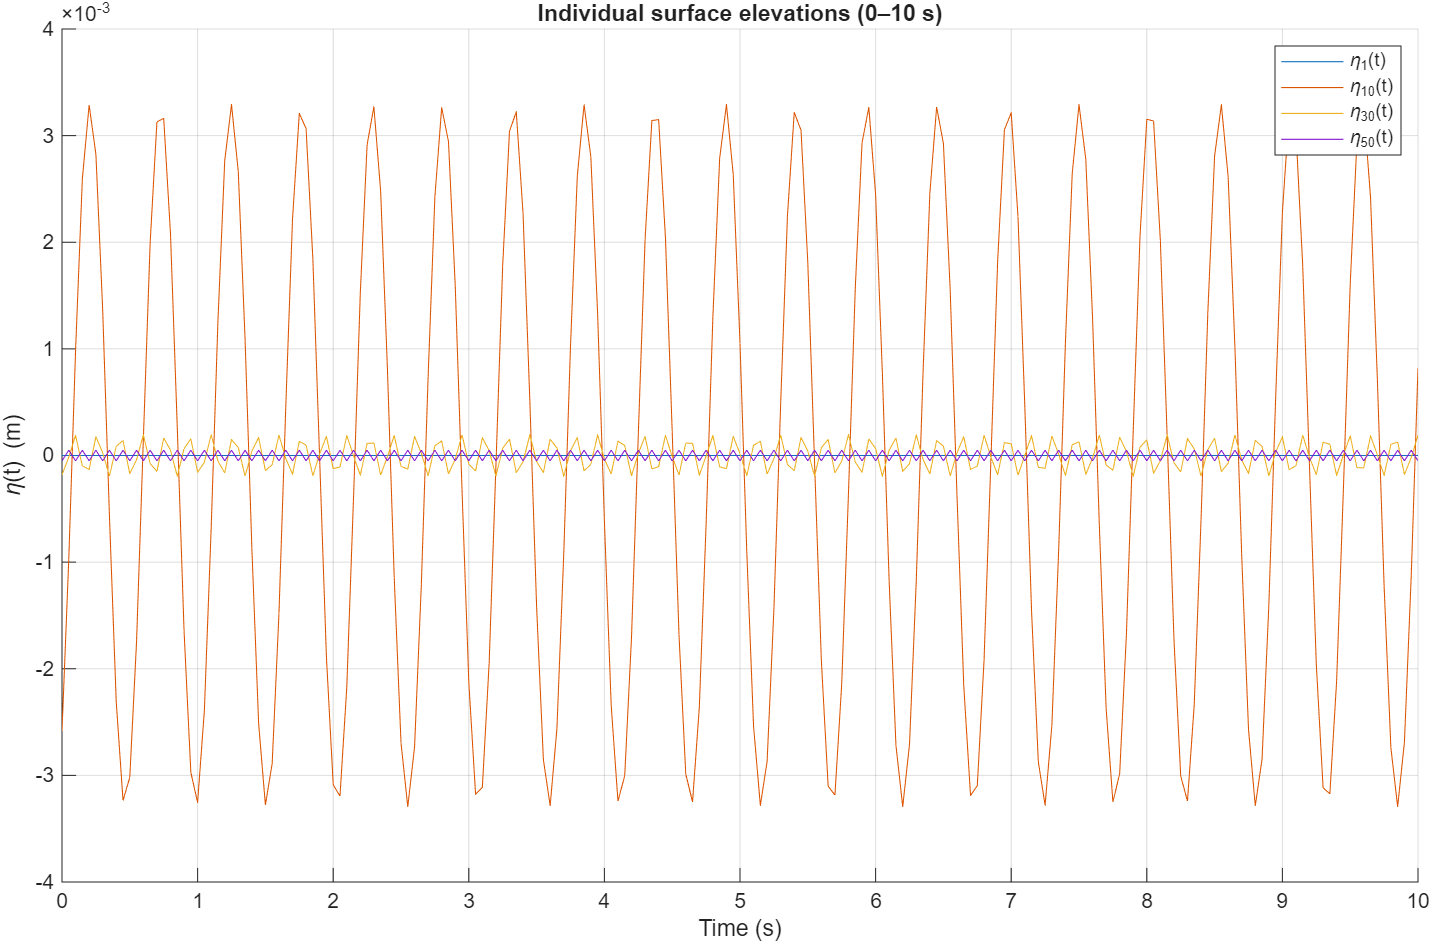
\includegraphics[width=0.8\textwidth]{partial_sums.png}
\caption{Surface elevation $\eta(t)$ for individual wave components of $i = 1, 10, 30, 50$.}
\label{fig:partial_sums}
\end{figure}

\autoref{fig:total_elevation} presents the total surface elevation $\eta(t)$ obtained by summing all 50 wave components over a period of 300 seconds. The plot exhibits irregular fluctuations and brief wave groups that form through the interaction of waves with similar frequencies.

\begin{figure}[H]
\centering
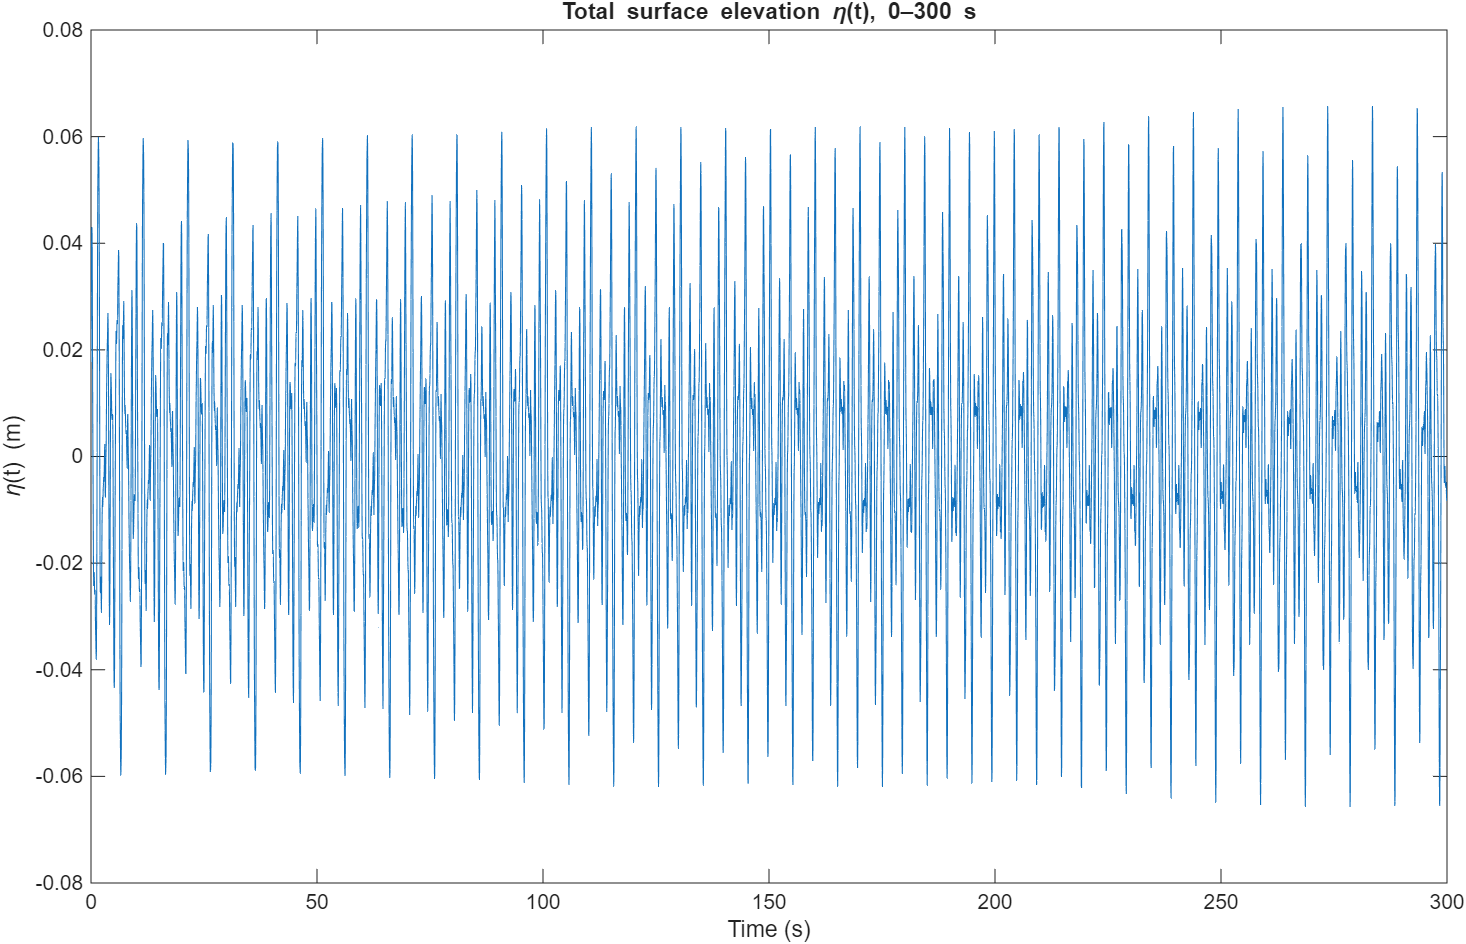
\includegraphics[width=0.8\textwidth]{eta_total.png}
\caption{Total surface elevation $\eta(t)$ over 0–300 s from the superposition of 50 components.}
\label{fig:total_elevation}
\end{figure}

To examine how the number of overlapping waves influences the simulated sea surface, the analysis was repeated for N=50, N=500 (\autoref{fig:n500}), and N=1000 (\autoref{fig:n1000}). Increasing N directly increases the number of individual wave components that are combined to form the total surface elevation. When only a small number of components are used, the sea surface is shaped by a few dominant frequencies, which produces a somewhat repetitive pattern. As more components are added, a larger range of frequencies interact simultaneously, and the resulting interference creates a surface that varies more irregularly in both height and period.

\begin{figure}[H]
\centering
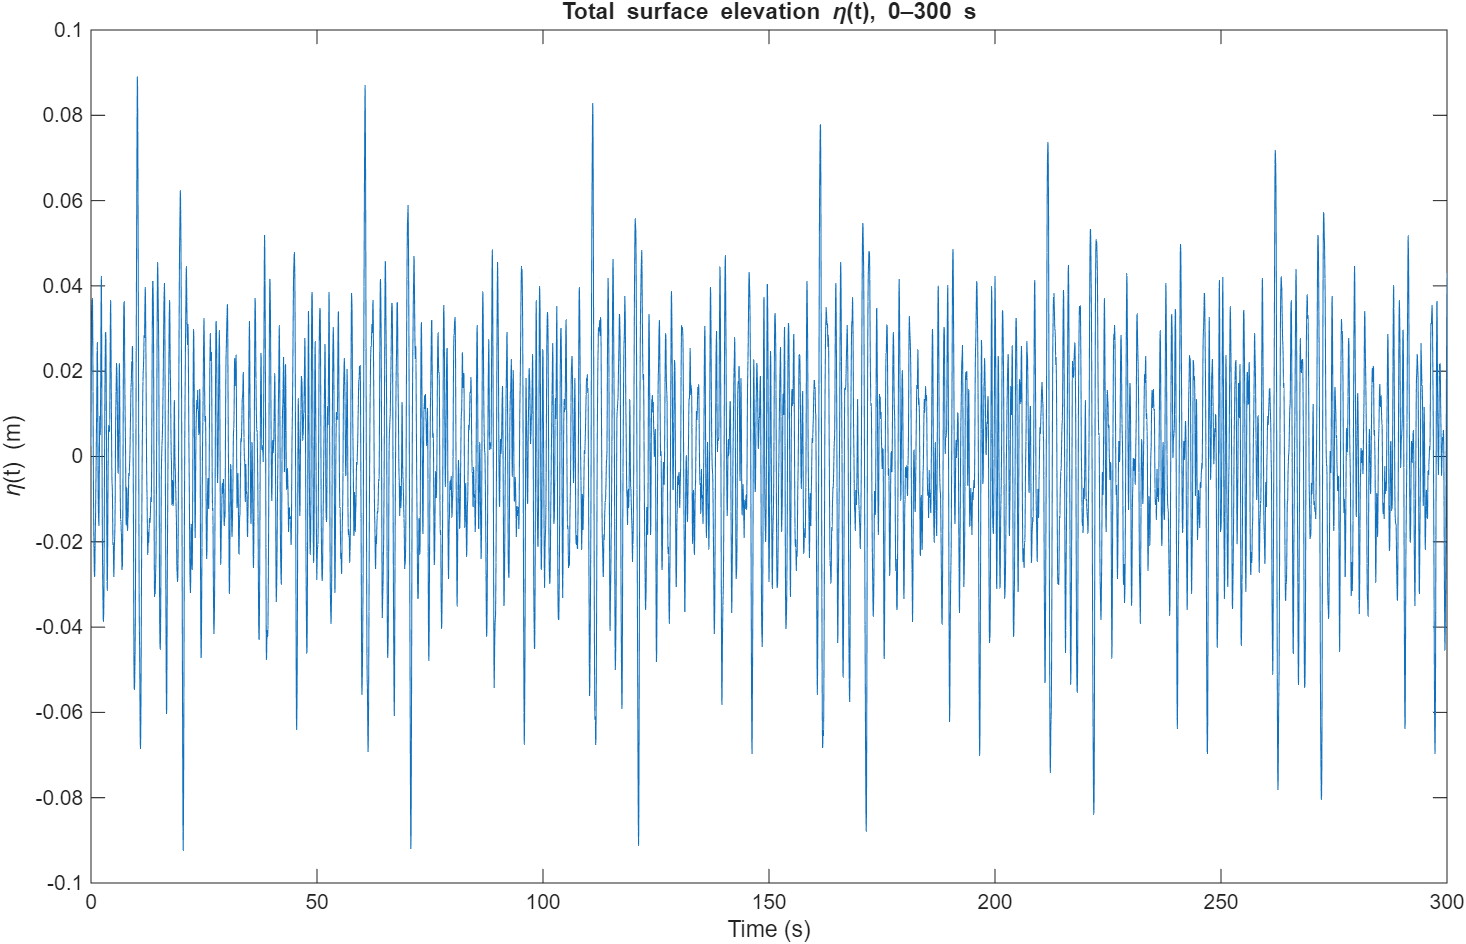
\includegraphics[width=0.75\textwidth]{n500.png}
\caption{Total surface elevation $\eta(t)$ over 0–300 s from the superposition of 500 components.}
\label{fig:n500}
\end{figure}

\begin{figure}[H]
\centering
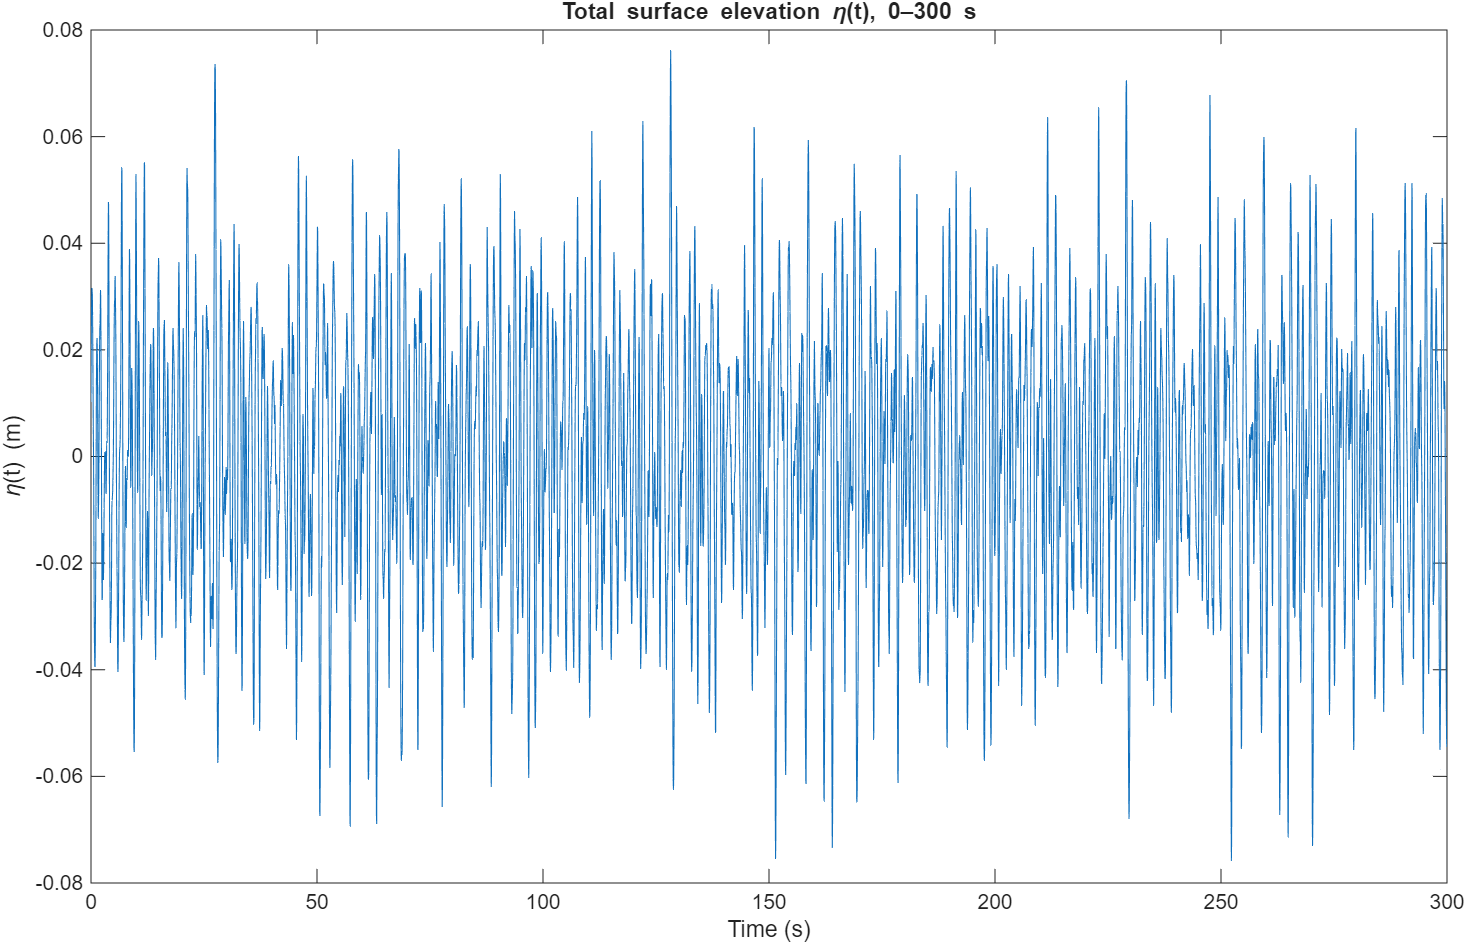
\includegraphics[width=0.75\textwidth]{n1000.png}
\caption{Total surface elevation $\eta(t)$ over 0–300 s from the superposition of 1000 components.}
\label{fig:n1000}
\end{figure}

\section{Conclusion and Discussion}

\hspace{0.5cm}In this study, a random sea surface was generated by adding together several sinusoidal wave components with different frequencies, amplitudes, and random phases. The Pierson-Moskowitz spectrum was used to determine the amplitude of each wave component based on its frequency. 

Increasing the number of components N directly increased the number of overlapping waves forming the total surface. For smaller N, the resulting time series appeared more repetitive. As N increased, more waves interacted, creating more interference and a surface that varied randomly over time.

This approach effectively simulates the complex and irregular nature of real sea surfaces, demonstrating how random wave fields can be constructed from known spectral characteristics. 
\newpage

\begin{thebibliography}{99}
\addcontentsline{toc}{section}{References}

\bibitem{Baykal2023}
Baykal, C. (2023). \textit{Lecture notes for CE 593 Statistical analysis in coastal engineering.} Middle East Technical University.

\end{thebibliography}
\newpage

\appendix
\section{Appendix}

\section*{MATLAB Code:}
\begin{lstlisting}[frame=single, numbers=left, style=Matlab-Pyglike]
%Parameters
h = 0.4; g = 9.81;
f = linspace(0.1, 10, 50);
N = numel(f);
df = f(2) - f(1);

T = 1 ./ f ;
L = arrayfun(@(t) dispersion_equation(t, h), T);
k = 2 * pi ./ L;

%Equations
n = 0.5 .* (1 + (2 * k * h) ./ (sinh(2 * k * h)));
phi = 0.5 .* tanh(k * h).^2 ./ n;
a = sqrt(2 * df .* (0.205 * 0.15^2 * 1.6^-4 .* f.^-5 .* exp(-0.75 * ...
    (1.6 .* f).^-4)) .* phi);
epsilon = 2 * pi * rand(1,N);

%Time ranges
t1 = 0 : 0.05 : 10;
t2 = 0 : 0.05 : 300;

%Part 1
eta1 = a.' .* cos(2 * pi * f.' .* t1 + epsilon.');

figure(1); hold on; grid on;
for idx = [1 10 30 50]
    plot(t1, eta1(idx,:), 'DisplayName', sprintf('\\eta_{%d}(t)', idx));
end

legend
title('Individual surface elevations (0-10 s)');
xlabel('Time (s)')
ylabel('\eta(t) (m)')

%Part 2
eta2 = sum(a.' .* cos(2 * pi * f.' .* t2 + epsilon.'), 1);

figure(2); grid on;
plot(t2, eta2);
title('Total surface elevation \eta(t), 0-300 s')
xlabel('Time (s)')
ylabel('\eta(t) (m)')
\end{lstlisting}


\end{document}